\documentclass[english,t]{beamer}
%\documentclass[finnish,english,handout]{beamer}

% Uncomment if want to show notes
% \setbeameroption{show notes}

\mode<presentation>
{
  %\usetheme{Warsaw}
  % % oder ...
  
  \setbeamercovered{invisible}
  % oder auch nicht
}
\setbeamertemplate{itemize items}[circle]
\setbeamercolor{frametitle}{bg=white,fg=navyblue}

\usepackage{graphicx}
\graphicspath{{./figs/}}
\usepackage[utf8]{inputenc}
\usepackage[T1]{fontenc}
\usepackage{times}
\usepackage{microtype}
\usepackage{epic,epsfig}
\usepackage{subfigure,float}
\usepackage{amsmath,amsfonts,amssymb}
\usepackage{inputenc}
\usepackage{babel}
\usepackage{afterpage}
\usepackage{eufrak}
\usepackage{amsbsy}
\usepackage{eucal}
\usepackage{rotating}
\usepackage{url}
\urlstyle{same}

\usepackage{natbib}
\bibliographystyle{apalike}

% \definecolor{hutblue}{rgb}{0,0.2549,0.6784}
% \definecolor{midnightblue}{rgb}{0.0977,0.0977,0.4375}
% \definecolor{hutsilver}{rgb}{0.4863,0.4784,0.4784}
% \definecolor{lightgray}{rgb}{0.95,0.95,0.95}
% \definecolor{section}{rgb}{0,0.2549,0.6784}
% \definecolor{list1}{rgb}{0,0.2549,0.6784}
 \definecolor{navyblue}{rgb}{0,0,0.5}
\renewcommand{\emph}[1]{\textcolor{navyblue}{#1}}

% \graphicspath{./pics}

\pdfinfo{            
  /Title      (Bayesian data analysis) 
  /Author     (Aki Vehtari) % 
  /Keywords   (Bayesian probability theory, Bayesian inference, Bayesian data analysis)
}


\parindent=0pt
\parskip=8pt
\tolerance=9000
\abovedisplayshortskip=0pt

\setbeamertemplate{navigation symbols}{}
\setbeamertemplate{headline}[default]{}
\setbeamertemplate{headline}[text line]{\insertsection}
\setbeamertemplate{footline}[frame number]


\def\o{{\mathbf o}}
\def\t{{\mathbf \theta}}
\def\w{{\mathbf w}}
\def\x{{\mathbf x}}
\def\y{{\mathbf y}}
\def\z{{\mathbf z}}

\DeclareMathOperator{\E}{E}
\DeclareMathOperator{\Var}{Var}
\DeclareMathOperator{\var}{var}
\DeclareMathOperator{\Sd}{Sd}
\DeclareMathOperator{\sd}{sd}
\DeclareMathOperator{\Gammad}{Gamma}
\DeclareMathOperator{\Invgamma}{Inv-gamma}
\DeclareMathOperator{\Bin}{Bin}
\DeclareMathOperator{\Bernoulli}{Bernoulli}
\DeclareMathOperator{\Negbin}{Neg-bin}
\DeclareMathOperator{\Poisson}{Poisson}
\DeclareMathOperator{\Beta}{Beta}
\DeclareMathOperator{\logit}{logit}
\DeclareMathOperator{\N}{N}
\DeclareMathOperator{\normal}{normal}
\DeclareMathOperator{\U}{U}
\DeclareMathOperator{\BF}{BF}
\DeclareMathOperator{\Invchi2}{Inv-\chi^2}
% \DeclareMathOperator{\Pr}{Pr}
\def\euro{{\footnotesize \EUR\, }}
\DeclareMathOperator{\rep}{\mathrm{rep}}


% ============
% Otsikko sivu
% ============

\title[]{Bayesian data analysis}
\subtitle{}

\author{Aki Vehtari}

\institute[  Aalto]{}

\begin{document} 

\begin{frame}{Benefits of integration and prior}

  \vspace{-0.5\baselineskip}
  Example: $n=10, y=10$ - uniform vs Beta(2,2) prior
  \begin{center}
  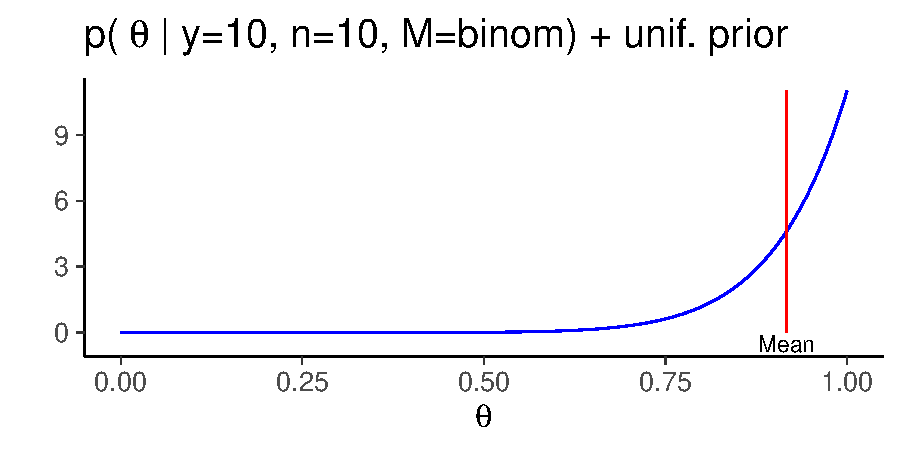
\includegraphics[width=7.8cm]{dbbeta10a.pdf}\\
  \uncover<2>{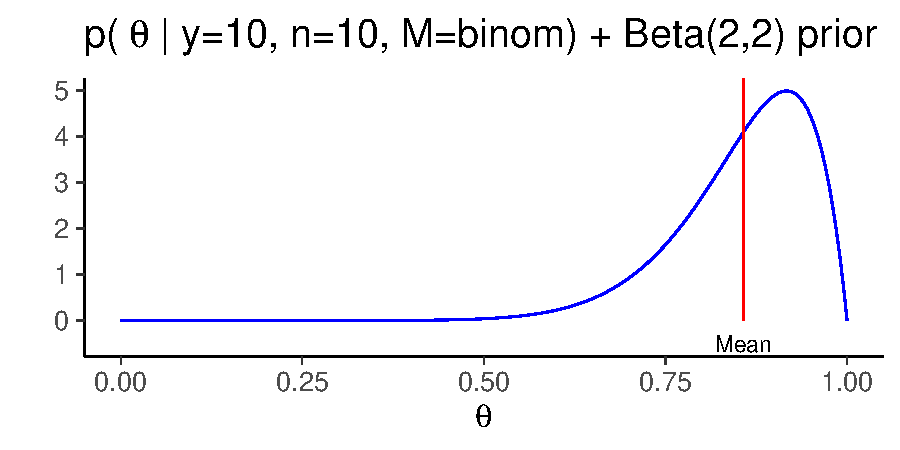
\includegraphics[width=7.8cm]{dbbeta10b.pdf}}
  \end{center}

\end{frame}

\begin{frame}{Benefits of integration: Gaussian process example}

  Simulated data of $g$ forces in a motorcycle accident

  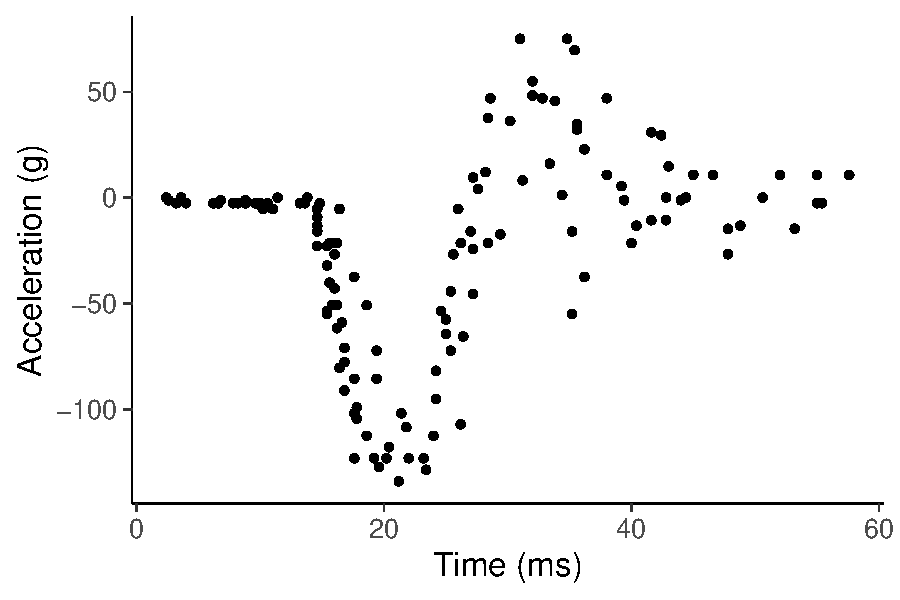
\includegraphics[width=11cm]{motorcycle_data.pdf}
  
\end{frame}

\begin{frame}{Benefits of integration: Gaussian process example}

  \begin{itemize}
  \item<+-> Gaussian process is a hierarchical normal model with
    multivariate normal population prior, where the off-diagonal
    covariances are determined by similarity measure (in the this
    example distance)
    \begin{align*}
      y & \sim \mbox{normal}(f(x), \sigma)\\
      f & \sim GP(0, K_1)\\
      \sigma & \sim \mbox{normal}^{+}(0, 1),
    \end{align*}
  \item<+-> $K_1$ is a covariance matrix, defined by a covariance
    function, that has parameters lengthscale $l$ and magnitude
    $\sigma_f$
  \item<+-> Latent values $f$ can be integrated out analytically, and the
    remaining marginal posterior is 3 dimensional
  \end{itemize}
\end{frame}

\begin{frame}{Benefits of integration: Gaussian process example}

  Plenty of data: the mode of th posterior can be representative
  
  \only<1>{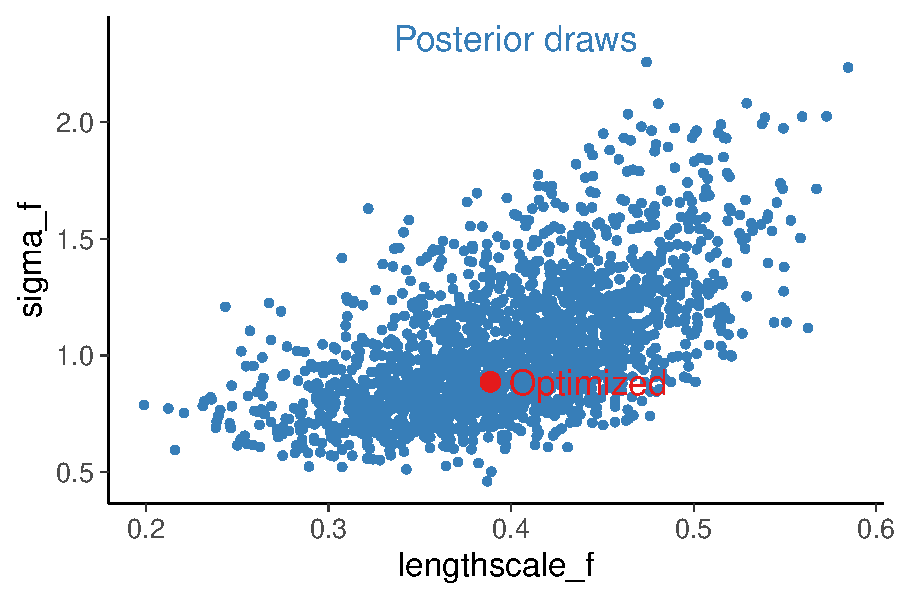
\includegraphics[width=11cm]{motorcycle_gpcovf_draws_optim_vs_mcmc.pdf}}
  \only<2>{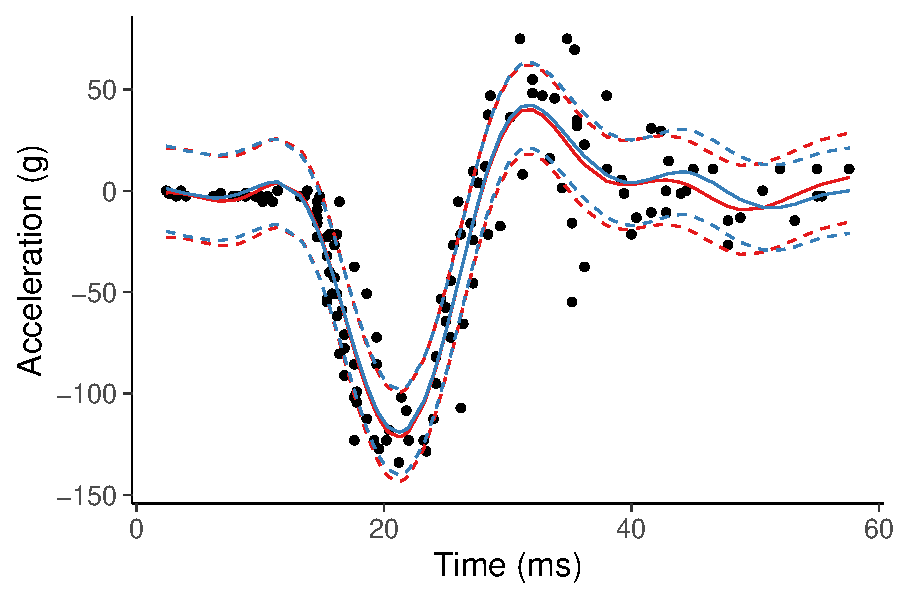
\includegraphics[width=11cm]{motorcycle_gpcovf_optim_vs_mcmc.pdf}}
  
\end{frame}

\begin{frame}{Benefits of integration: Gaussian process example}

  Small data: the mode of the posterior is not representative

    \only<1>{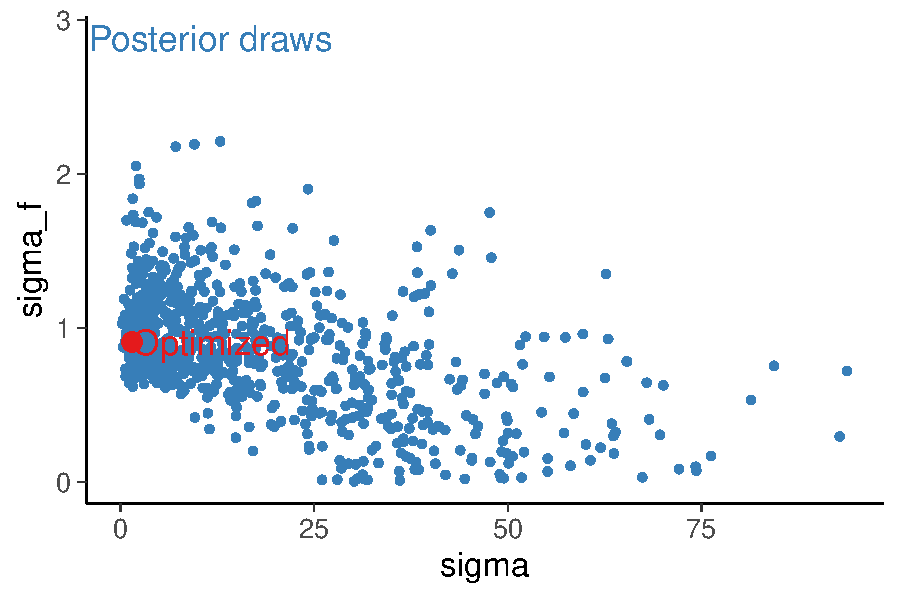
\includegraphics[width=11cm]{motorcycle_gpcovf_10p_draws_optim_vs_mcmc.pdf}}
  \only<2>{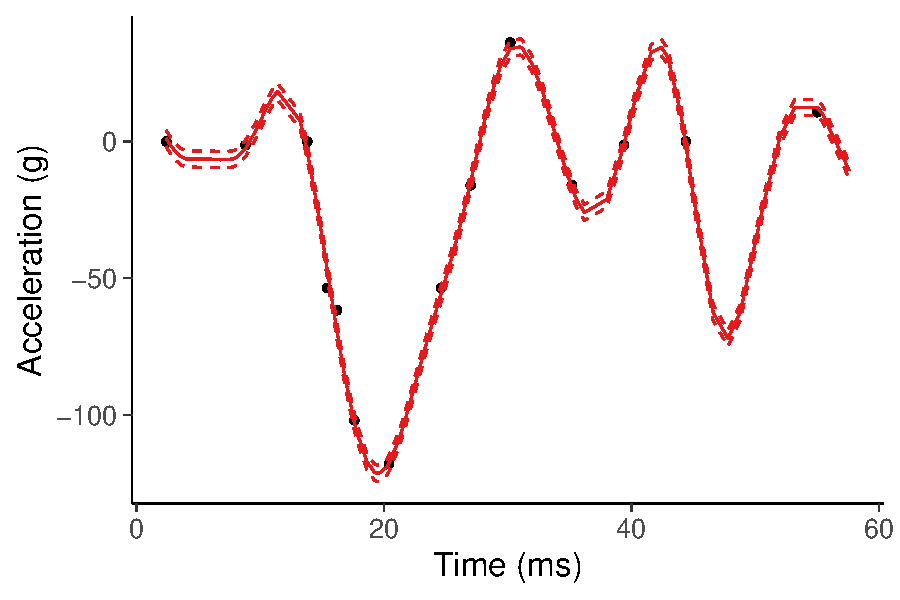
\includegraphics[width=11cm]{motorcycle_gpcovf_10p_optim.pdf}}
  \only<3>{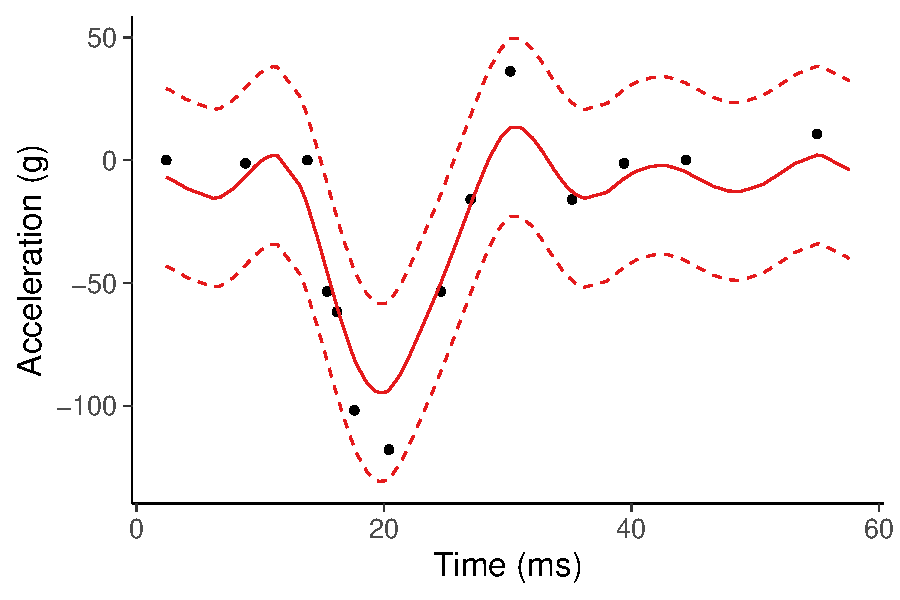
\includegraphics[width=11cm]{motorcycle_gpcovf_10p_mcmc.pdf}}
  \only<4>{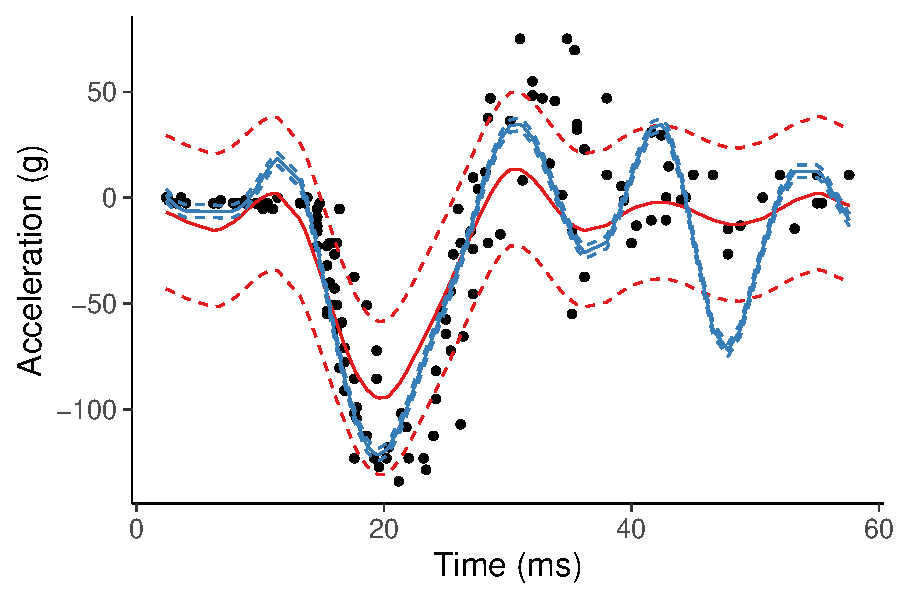
\includegraphics[width=11cm]{motorcycle_gpcovf_10p_optim_vs_mcmc.pdf}}

\end{frame}

\begin{frame}{Benefits of integration: Gaussian process example}
  
  \begin{itemize}
  \item<+-> More complex model, with time dependent residual variance
    $\exp(g(x))$
    \begin{align*}
      y & \sim \normal(f(x), \exp(g(x))\\
      f & \sim GP(0, K_1)\\
      g & \sim GP(0, K_2).
    \end{align*}
  \item<+-> Latent values can not be integrated out analytically, and
    the posterior is 270 dimensional
  \end{itemize}
  
\end{frame}

\begin{frame}{Benefits of integration: Gaussian process example}

  \only<1>{The mode of the posterior is not representative

    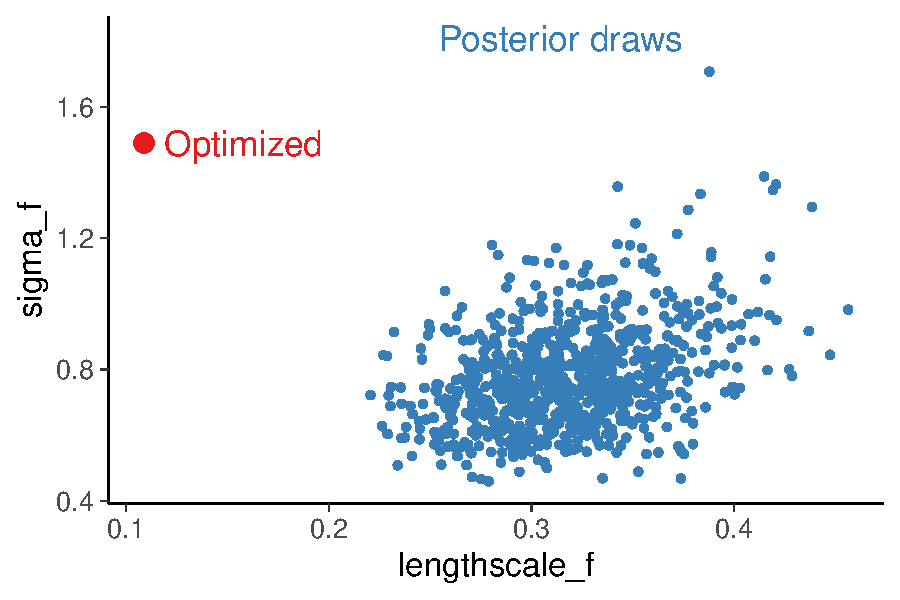
\includegraphics[width=11cm]{motorcycle_gpcovfg_draws_optim_vs_mcmc.pdf}}
  \only<2>{Optimization overfits

    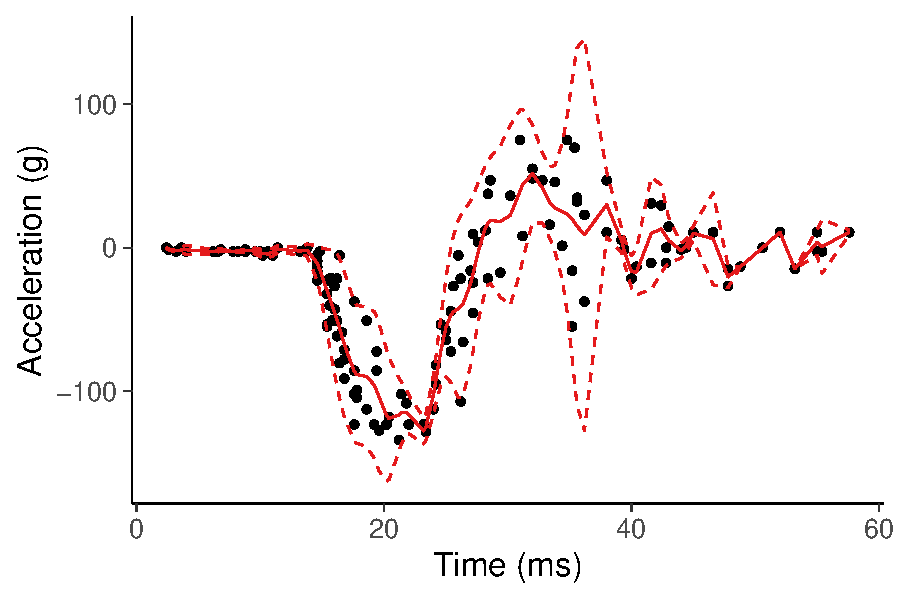
\includegraphics[width=11cm]{motorcycle_gpcovfg_optim.pdf}}
  \only<3>{Integration works well

    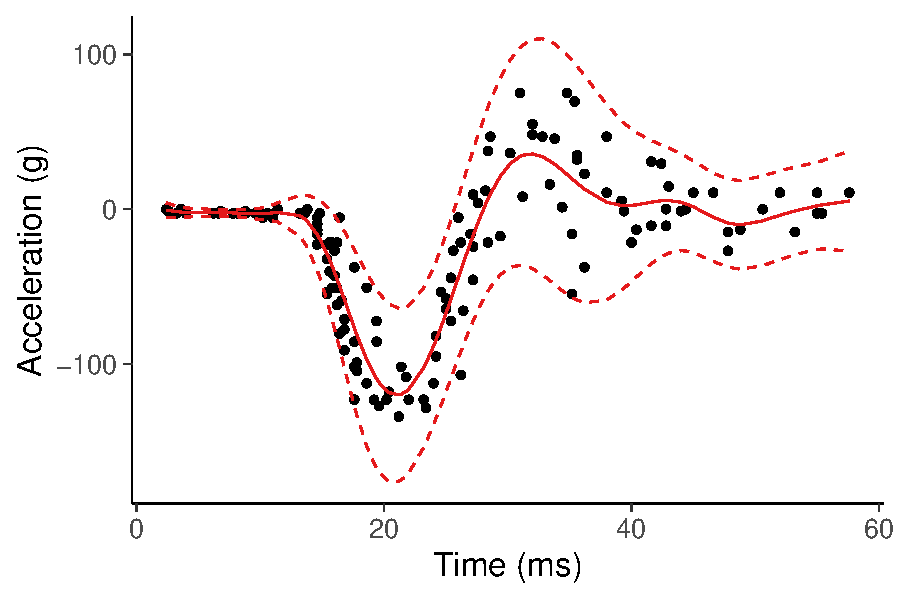
\includegraphics[width=11cm]{motorcycle_gpcovfg_mcmc.pdf}}

\end{frame}


\begin{frame}{Benefits of better priors: logistic regression}

  \begin{align*}
    y & \sim  \Bernoulli\left( \logit^{-1}(\alpha + \beta X )\right)
  \end{align*}
  where $\alpha$ is a scalar intercept,\\ and $\beta$ is a vector of
  coefficients
  
\end{frame}
\begin{frame}{Model selection is needed to avoid overfitting?}

  logistic regression: 30 \textbf{completely irrelevant} variables, \\100
  observations
  
  \only<2>{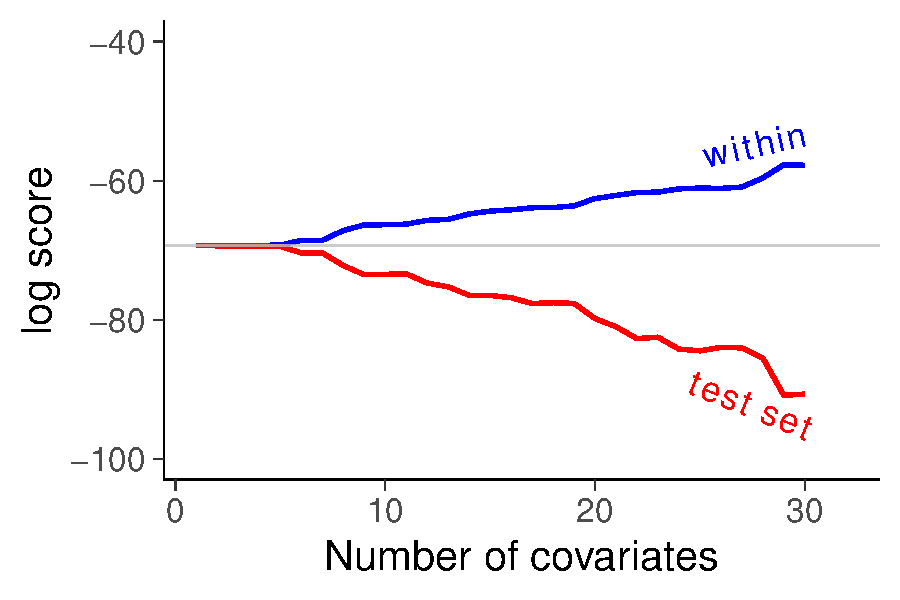
\includegraphics[width=10cm]{irrelevant_N.pdf}}

\end{frame}

\begin{frame}{Prior on parameters vs predictions}

N(0,3) prior on each coefficient\\
\only<1>{1 variable\\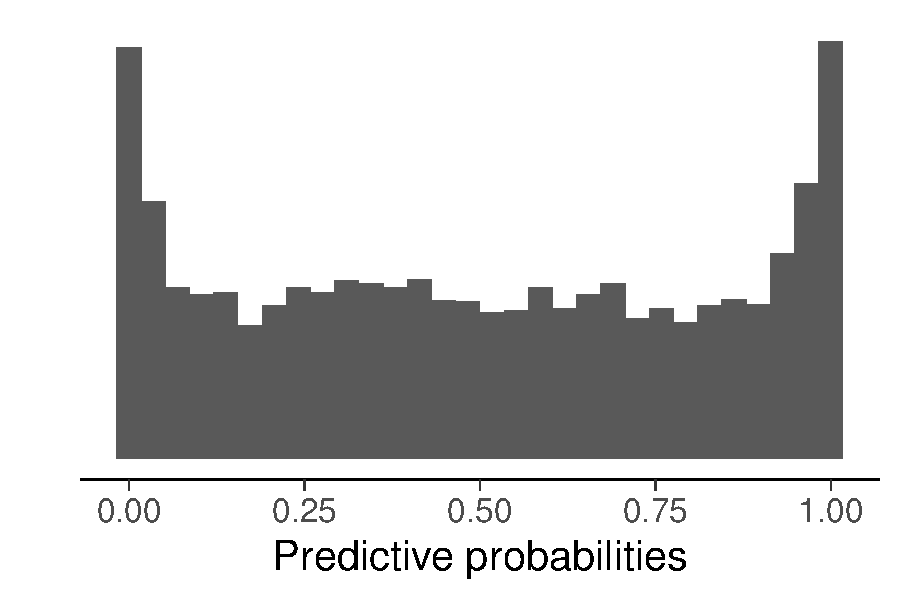
\includegraphics[width=9cm]{prior_N_1.pdf}}
\only<2>{2 variables\\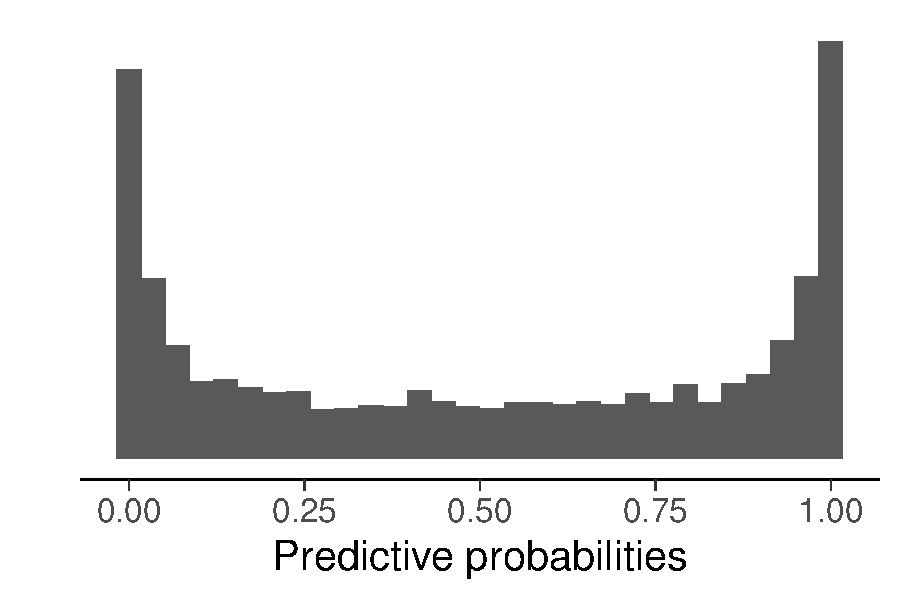
\includegraphics[width=9cm]{prior_N_2.pdf}}
\only<3>{3 variables\\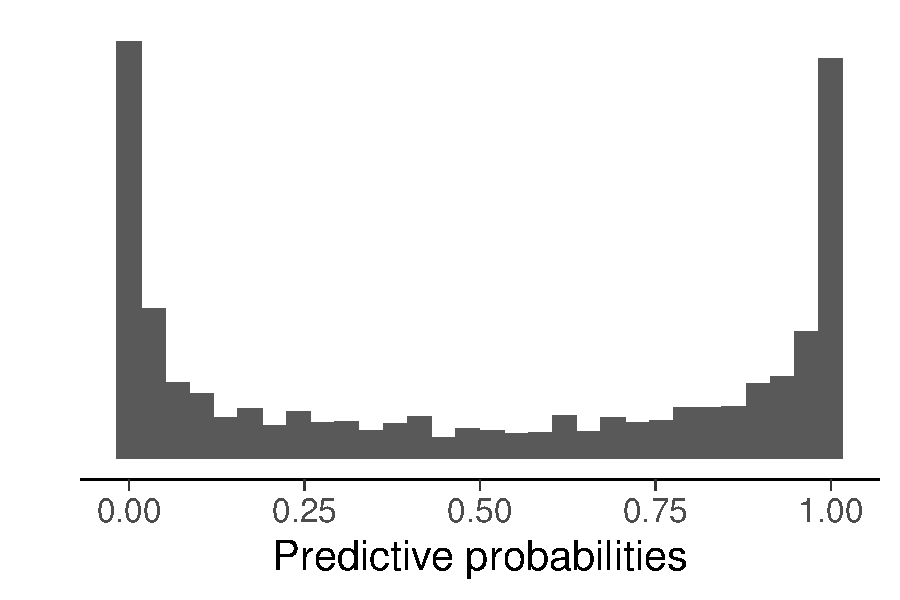
\includegraphics[width=9cm]{prior_N_3.pdf}}
\only<4-5>{30 variables\\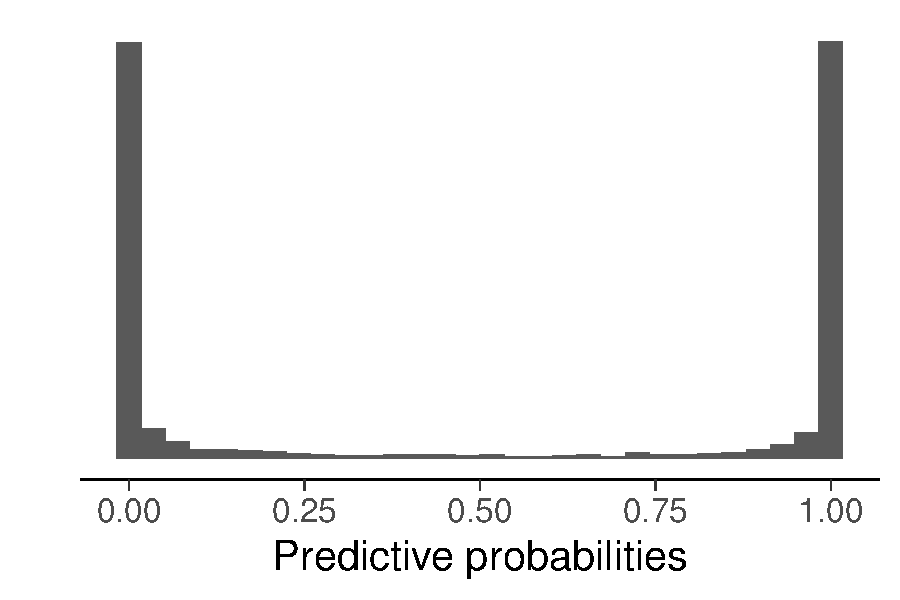
\includegraphics[width=9cm]{prior_N_30.pdf}}

\only<5>{A weak prior on parameters can be a strong prior on predictions}

\end{frame}

\begin{frame}{Better priors}

N(0,$\frac{1}{\sqrt{p}}$) prior on each coefficient\\
\only<1>{1 variable\\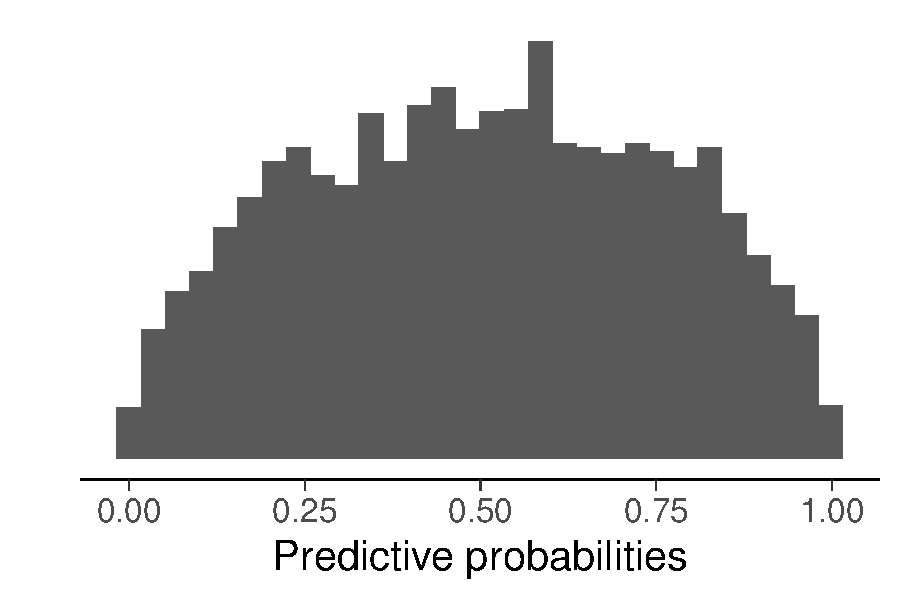
\includegraphics[width=9cm]{prior_Ns_1.pdf}}
\only<2>{2 variables\\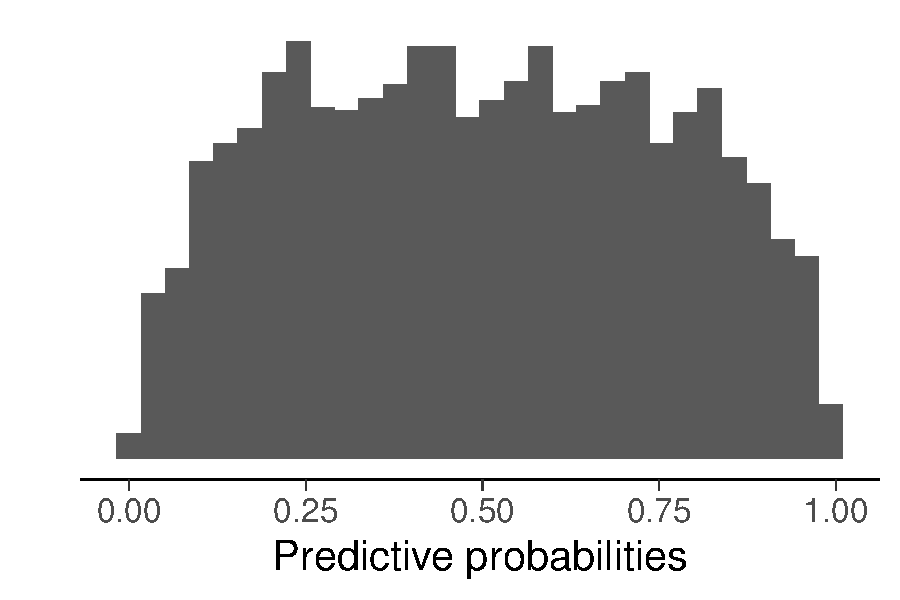
\includegraphics[width=9cm]{prior_Ns_2.pdf}}
\only<3>{3 variables\\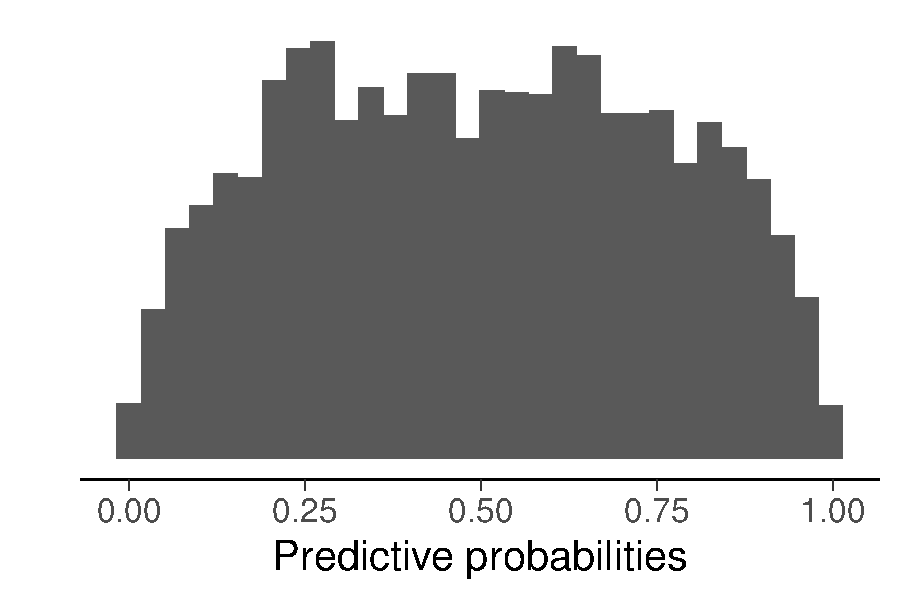
\includegraphics[width=9cm]{prior_Ns_3.pdf}}
\only<4-5>{30 variables\\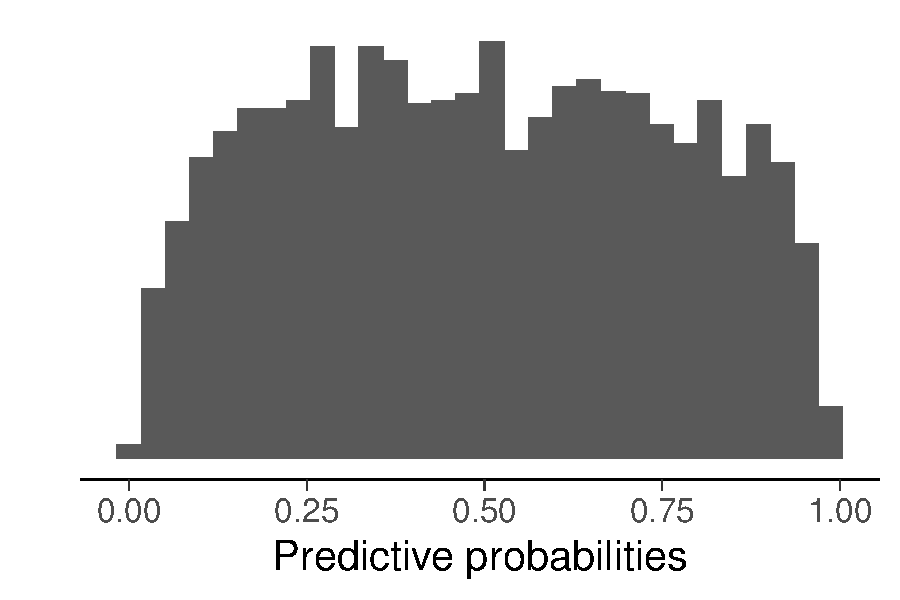
\includegraphics[width=9cm]{prior_Ns_30.pdf}}

\only<5>{Prior on predictions (almost) fixed when the model gets bigger}
  
\end{frame}

\begin{frame}{Better priors, no overfitting}

  logistic regression: 30 \textbf{completely irrelevant} variables, \\100
  observations
  
  \only<1>{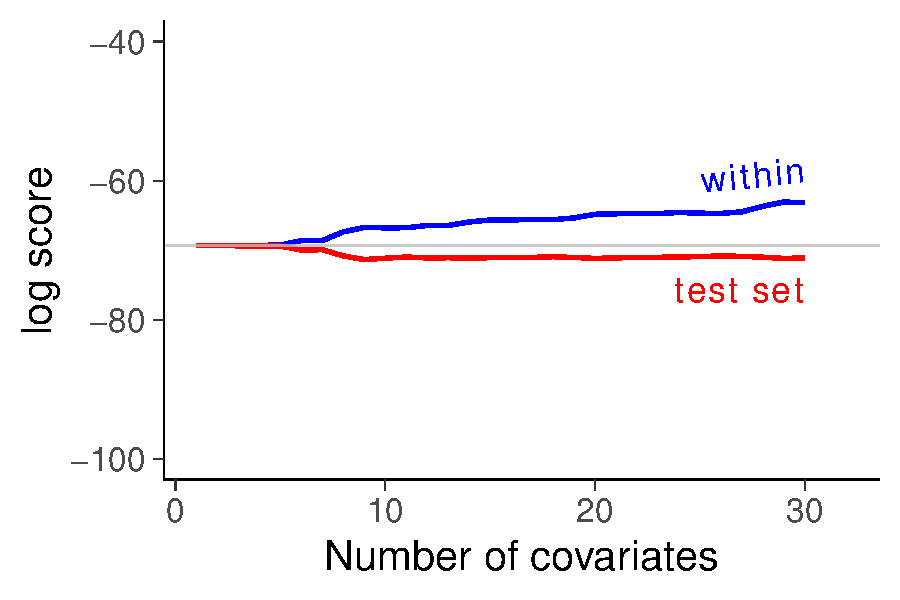
\includegraphics[width=10cm]{irrelevant_Ns.pdf}}
%  \only<2>{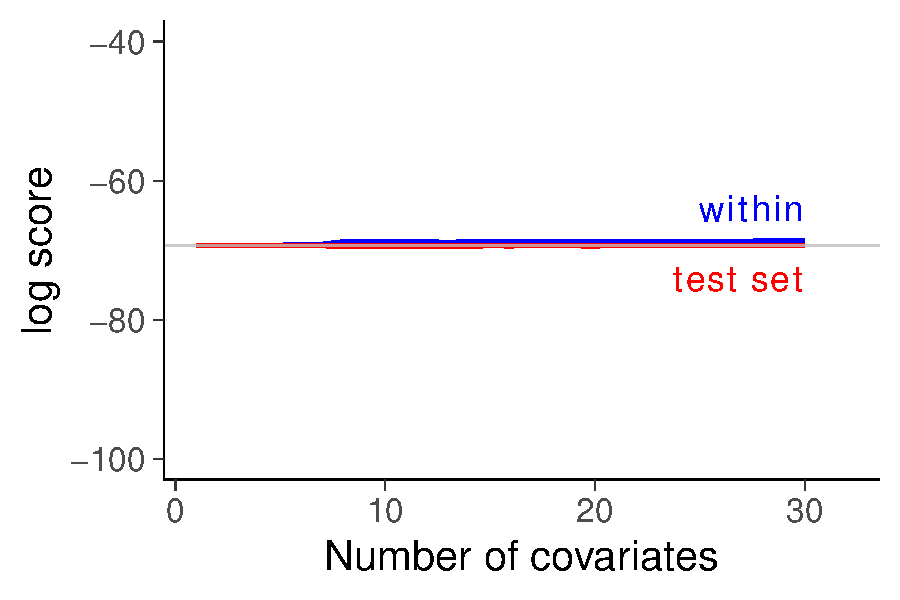
\includegraphics[width=10cm]{irrelevant_RHS.pdf}}
  
\end{frame}

\begin{frame}{Many weak effects, wide prior on parameters}

  logistic regression: 30 \textbf{weakly relevant} variables, \\100
  observations, wide prior
  
  \only<2>{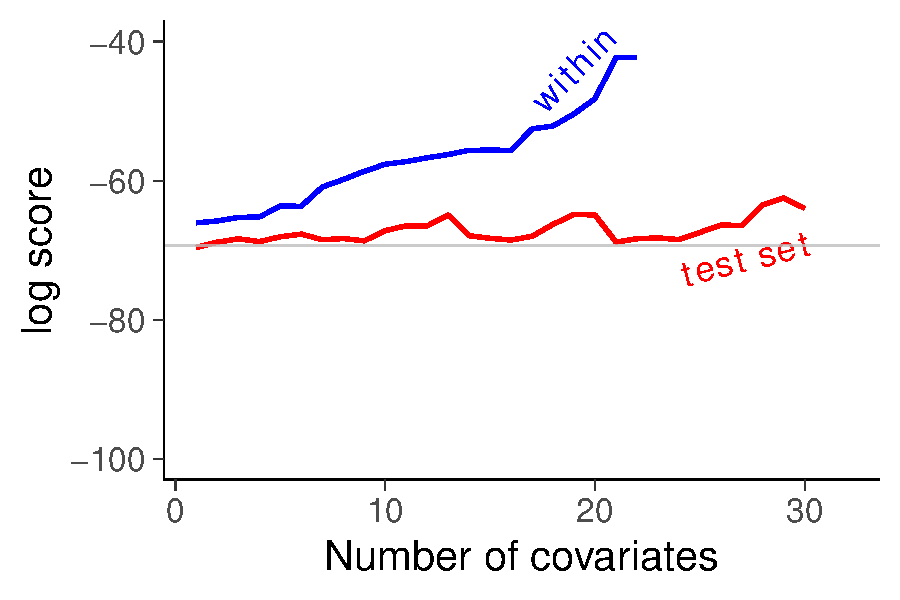
\includegraphics[width=10cm]{weak_N.pdf}}

\end{frame}

\begin{frame}{Many weak effects, better prior}

  logistic regression: 30 \textbf{weakly relevant} variables, \\100
  observations, better prior
  
  \only<1>{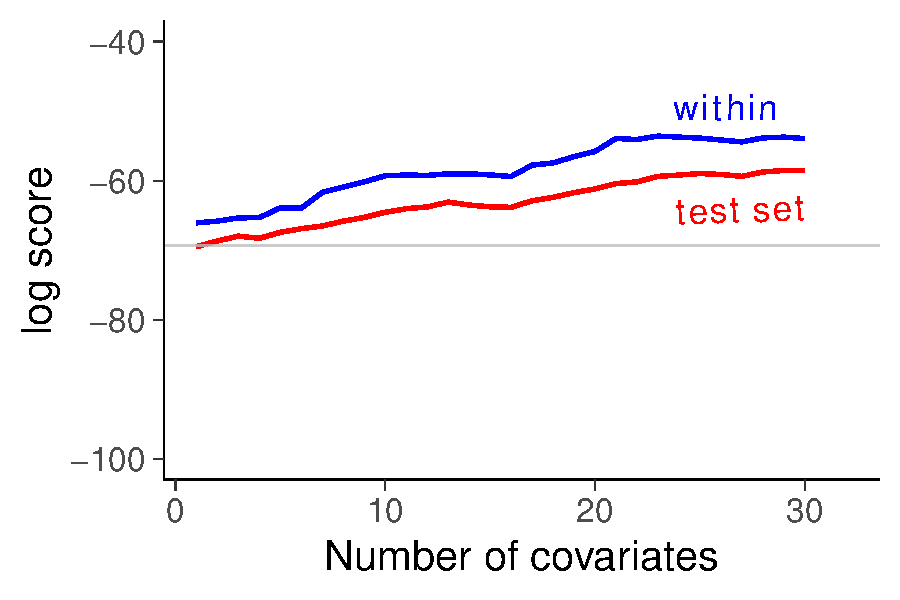
\includegraphics[width=10cm]{weak_Ns.pdf}}

\end{frame}

\begin{frame}{Correlating variables, wide prior on parameters}

  logistic regression: 30 \textbf{correlating relevant} variables, \\100
  observations
  
  % \only<1>{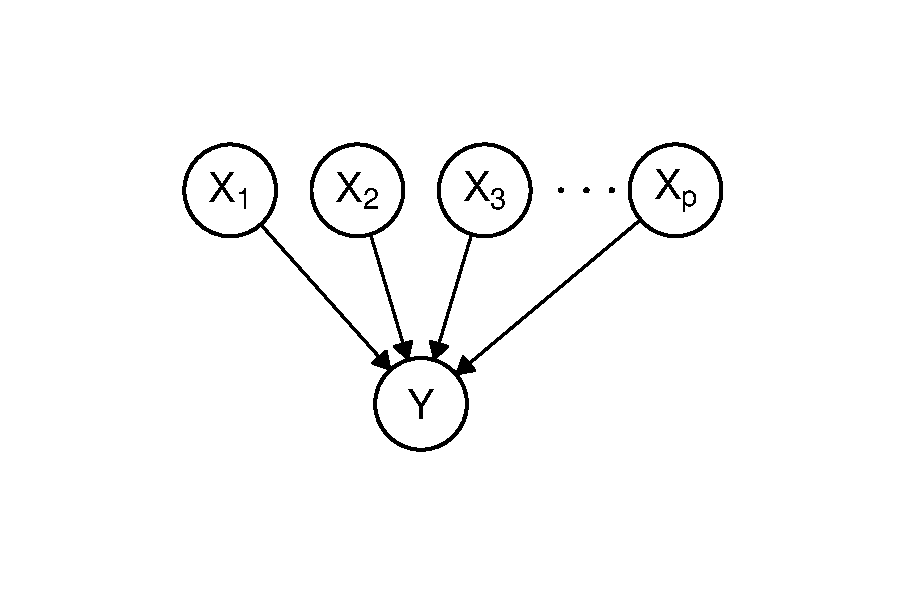
\includegraphics[width=9cm]{fig/simple.pdf}}
  \only<2>{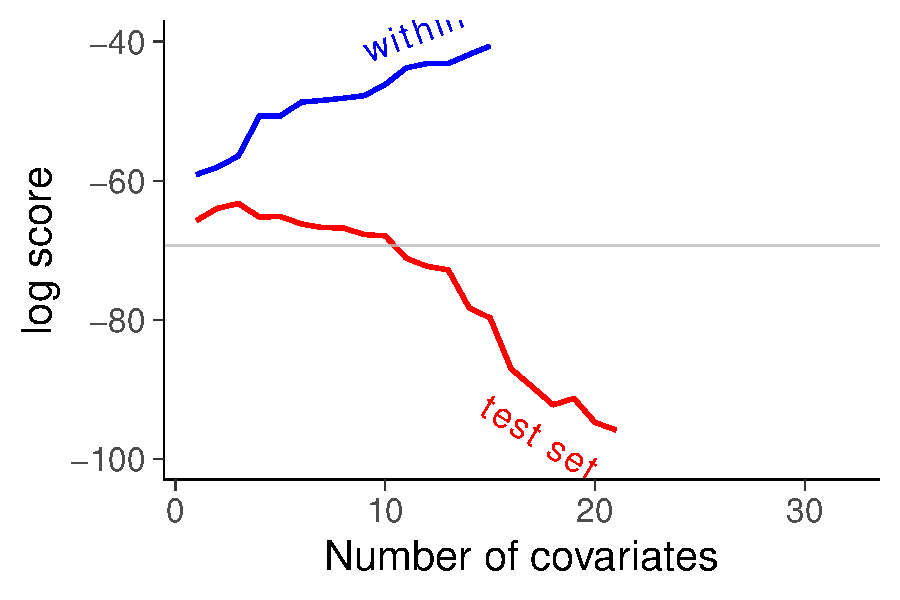
\includegraphics[width=10cm]{correlating_N.pdf}}

\end{frame}

\begin{frame}{Correlating variables, better prior}

  logistic regression: 30 \textbf{correlating relevant} variables, \\100
  observations
  
  \only<1>{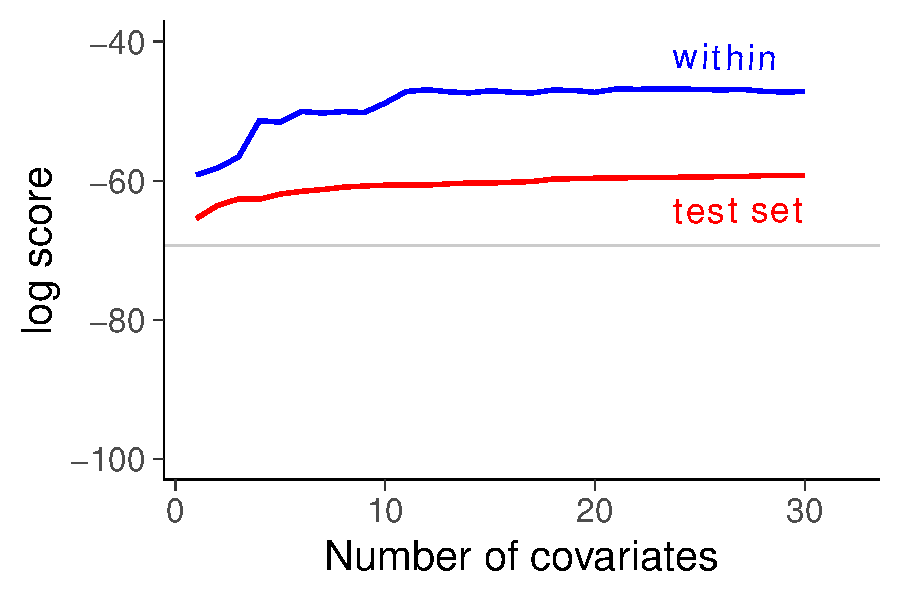
\includegraphics[width=10cm]{correlating_Ns.pdf}}

\end{frame}

\begin{frame}{Benefits of integration and prior}

  \begin{itemize}
  \item Integration helps to avoid overfitting
  \item Integration is not able to counter bad priors
  \end{itemize}
  
\end{frame}

\end{document}

%%% Local Variables: 
%%% TeX-PDF-mode: t
%%% TeX-master: t
%%% End: 
